\section{Disproving the Conjectures}
\label{section_counter_example_main_polytope_study_disproving_conjecture}
In this section we disprove Conjectures \ref{conjecture_LP_finds_STT_vertex} and \ref{conjecture_LP_rounding_finds_opt_STT}. We first disprove Conjecture~\ref{conjecture_LP_finds_STT_vertex} by showing a specific non-integer vertex for a specific topology and frequencies such that this vertex is strictly better than any STT (Section~\ref{subsection_specific_counter_example}). Then we generalize the discussion to elaborate further on our technique for finding this specific example and multiple others (Section~\ref{subsection_general_counter_exaple}), and study the integrality gap of the LP (Section~\ref{subsection_integrality_gap}). Finally, in Section~\ref{subsection_approximation_ratio} we disprove Conjecture~\ref{conjecture_LP_rounding_finds_opt_STT} and show that the proposed rounding scheme may result in a sub-optimal STT. There, we also  give a lower bound on the approximation-ratio for this specific rounding scheme.

\subsection{Specific Counter Example: Strictly Better Fractional Vertex}
\label{subsection_specific_counter_example}

In this section we provide an explicit example for a topology and frequencies such that the LP solution for it is strictly better than any solution induced by a search tree. The topology and frequencies were found using computer search (Appendix~\ref{appendix_section_code}), more details follow in Section~\ref{subsection_general_counter_exaple}. 
In this section we provide
a proof that the solution we found 
is a non-integer feasible solution to the LP, such that any other integer solution that is induced by a search tree is strictly worse.

%Regardless of anything that could go wrong with code such as possible bugs, numeric errors or incomplete exhaustive search, the example in this section is proven explicitly to be a non-integer feasible solution to the LP, such that any other integer solution that is induced by a search tree is strictly worse.

\begin{definition}[Terminology]
\label{definition_long_star}
For ease of reference, we define the following terminology. Let $U$ be a tree over $n=7$ nodes such that nodes $1$ to $5$ form a path in the natural order, with additional edges $(3,6)$ and $(6,7)$. This is also the tree in Figure~\ref{figure_topology_to_stt_example}, and $U_{(7,3)}$ in Figure~\ref{figure_all_trees_up_to_n8}. We refer to $U$ as a \emph{long star}, with three \emph{legs}. We refer to $3$ as its center, to $1,5,7$ as leaves, and to $2,4,6$ as mid-nodes.
\end{definition}

\begin{theorem}
\label{theorem_non_integer_optimum_long_star}
    Let $U$ be a long-star (Definition~\ref{definition_long_star}). Let $f = \frac{1}{23} [3,2,0,2,3,3,10]$ be the frequencies vector, i.e., such that $f_i$ is the frequency of querying node $i$. Then there is a feasible solution $P$ with depth coordinates $P_D = [2,2,4.5,2,2,1.5,0.5]$ that is strictly better for the LP with weights $f$ compared to any feasible point induced by an STT over $U$.
\end{theorem}

We note before the proof:
\begin{enumerate}
    \item Theorem~\ref{theorem_non_integer_optimum_long_star} holds even when we require a vector of strictly positive frequencies. Indeed, we can perturb $f_3$ by some $\epsilon > 0$ and still maintain a strictly-better feasible solution.
    
    \item $P$ is in fact a vertex, as determined by our LP-solver code. That being said, Theorem~\ref{theorem_non_integer_optimum_long_star} does not require $P$ to be a vertex, just that its value is strictly better than any STT.
\end{enumerate}


\begin{figure}[ht]
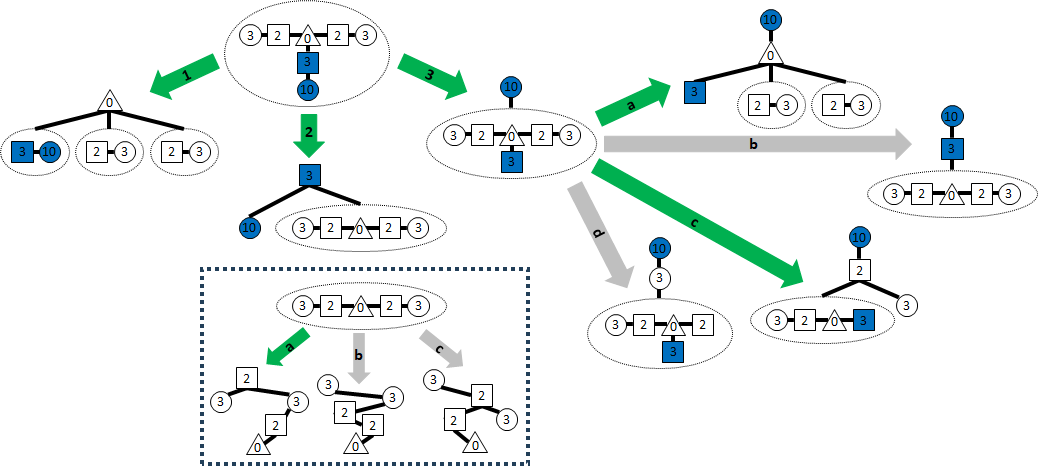
\includegraphics[width=1.0\textwidth]{figure_case_analysis.png}
\caption{\footnotesize{Visualization of the case analysis in proving Theorem~\ref{theorem_non_integer_optimum_long_star}. The blue nodes emphasize the heaviest leg, weights are written within the nodes, and the shapes emphasize the type of each node in the topology: center (triangle), mid-node (square), leaf (circle). A dashed ellipse indicates that the STT for this component is undetermined, yet. The numbers and letters within the arrows correspond to the cases of the proof. Green arrows lead to an STT that minimizes the LP among STTs, gray arrows lead to sub-optimal solutions.}}
\label{figure_case_analysis}
\end{figure}

\begin{proof}
For convenience, we scale the frequencies back to integer weights and use the vector $w = 23 \cdot f = [3,2,0,2,3,3,10]$.
%Its effect on the LP is just scaling, so nothing changes.
We divide the proof to two parts. First we describe all the coordinates of $P$ and verify its feasibility. Then we case-analyze the best possible value of a search tree, to show that it is strictly worse than the value of $P$.

\textbf{The solution $P$:} We present the values of the variables of $P$ in Figure~\ref{figure_explicit_counter_example}, where the $X_{ij}$ variables form a matrix $X$ (note that the variables $X_{ii}$ do not exist, so these entries are marked by '.'). The $D_i$'s are written below $X$, as they are the sums of the columns of $X$, and $Z_{kij}$ are to the side of $X$. The figure also verifies feasibility for each of the (in)equalities. The weighted depth of $P$ is: $P_D \cdot w = [2,2,4.5,2,2,1.5,0.5] \cdot [3,2,0,2,3,3,10] = 6+4+0+4+6+4.5+5=29.5$.


\begin{figure}[ht]
    {\footnotesize
    \begin{subfigure}{0.9\textwidth}
        \begin{equation}
        \label{equation_vertex_opt_values}
        \begin{bmatrix}
            X \\
            \hline
            D
            \end{bmatrix}
        =
            \begin{bmatrix}
            . & h & h & 0 & 0 & 0 & 0 \\
            h & . & 1 & h & h & h & 0 \\
            0 & 0 & . & 0 & 0 & 0 & 0 \\
            h & h & 1 & . & h & h & 0 \\
            0 & 0 & h & h & . & 0 & 0 \\
            h & h & 1 & h & h & . & h \\
            h & h & h & h & h & h & . \\
            \hline
            2 & 2 & 4.5 & 2 & 2 & 1.5 & 0.5 \\
            \end{bmatrix}
        ; Z:
        \begin{bmatrix*}[l]
            Z_{213}=Z_{214}=Z_{215}=Z_{415}=Z_{216}=Z_{617}=h \\
            Z_{314}=Z_{315}=Z_{316}=Z_{217}=Z_{317}=0 \\
    
            Z_{425}=Z_{627}=h \\
            Z_{324}=Z_{325}=Z_{326}=Z_{327}=0 \\
        
            Z_{435}=Z_{637}=Z_{647}=Z_{456}=Z_{657}=h \\
            Z_{346}=Z_{347}=Z_{356}=Z_{357}=Z_{457}=0 \\
        \end{bmatrix*}
        \end{equation}
        
    \end{subfigure}
    }
    
    {\footnotesize
    \begin{subfigure}{0.9\textwidth}
        \begin{equation}
        \label{equation_vertex_opt_inequalities}
        \begin{split} % See about split and alignment: https://www.overleaf.com/learn/latex/Aligning_equations_with_amsmath
        &
            \begin{bmatrix*}[l]
            X_{12}+X_{21} \\
            X_{13}+X_{31} + Z_{213} \\
            X_{14}+X_{41} + Z_{214} + Z_{314} \\
            X_{15}+X_{51} + + Z_{215} + Z_{315} + Z_{415} \\
            X_{16}+X_{61} + Z_{216} + Z_{316} \\
            X_{17}+X_{71} + Z_{217} + Z_{317} + Z_{617} \\
            X_{23}+X_{32} \\
            X_{24}+X_{42} + Z_{324} \\
            X_{25}+X_{52} + Z_{325}+ Z_{425} \\
            X_{26}+X_{62} + Z_{326} \\
            X_{27}+X_{72} + Z_{327} + Z_{627} \\
            \end{bmatrix*}
        =
            \begin{bmatrix*}[l]
            h+h \\
            0+h+h \\
            0+h+h+0\\
            0+0+h+0+h\\
            0+h+h+0\\
            0+h+0+0+h\\
            1+0\\
            h+h+0\\
            h+0+0+h\\
            h+h+0\\
            0+h+0+h\\
            \end{bmatrix*}
        ;
            \begin{bmatrix*}[l]
            X_{34}+X_{43} \\
            X_{35}+X_{53} + Z_{435} \\
            X_{36}+X_{63} \\
            X_{37}+X_{73} + Z_{637} \\
            X_{45}+X_{54} \\
            X_{46}+X_{64} + Z_{346} \\
            X_{47}+X_{74} + Z_{347}+ Z_{647} \\
            X_{56}+X_{65} + Z_{356}+ Z_{456} \\
            X_{57}+X_{75} + Z_{357}+ Z_{457}+ Z_{657} \\
            X_{67}+X_{76} \\
            \end{bmatrix*}
        =
            \begin{bmatrix*}[l]
            0+1\\
            0+h+h\\
            0+1 \\
            0+h+h\\
            h+h \\
            h+h+0 \\
            0+h+0+h\\
            0+h+0+h\\
            0+h+0+0+h\\
            h+h\\
            \end{bmatrix*}
        \\
        &
            \begin{bmatrix*}[l]
            Z_{213}=Z_{214}=Z_{215}=Z_{216} \\
            Z_{617}=Z_{627}=Z_{637}=Z_{647}=Z_{657} \\
            Z_{415}=Z_{425}=Z_{435}=Z_{456} \\
            \end{bmatrix*}
        =
        h
        \le
            \begin{bmatrix*}[l]
            X_{21},X_{23},X_{24},X_{25},X_{26} \\
            X_{61},X_{62},X_{63},X_{64},X_{65},X_{67} \\
            X_{41},X_{42},X_{43},X_{45},X_{46} \\
            \end{bmatrix*}
        =
            \begin{bmatrix*}[l]
            h,1,h,h,h \\
            h,h,1,h,h,h \\
            h,h,1,h,h \\
            \end{bmatrix*}
        \end{split}
        \end{equation}
    \end{subfigure}
    }
    
\caption{\footnotesize{The vertex $P$. (Eq.~\ref{equation_vertex_opt_values}) The values of $P$, where $h = \frac{1}{2}$ (short for half). The $Z$ variables are separated to three pairs of rows (of values $0$ and $h$). The first pair covers all $Z_{k1j}$, the next pair covers all $Z_{k2j}$ and the last pair covers $Z_{kij}$ for $i \ge 3$. The vector $D$ is a column-sum of the matrix $X$. (Eq.~\ref{equation_vertex_opt_inequalities}) Proof of feasibility, listing all the ancestry-inequalities. Inequalities of the form $Z_{kij} \le X_{ki},X_{kj}$ are verified in ``bulk'' (only non-trivial for $Z_{kij} > 0$).}}
\label{figure_explicit_counter_example}
\end{figure}

\textbf{Case analysis of all search trees:}
The number of STTs over $U$ is too large for hand verification. There are $662$ in total, but  $U$ is symmetric, and $w$ is also mostly symmetric. This enables us to reduce the analysis to a handful of cases. We emphasize that in the following discussion, the quality of an STT is considered with respect to $w = [3,2,0,2,3,3,10]$, and that the depths start from $0$ (root) (see Remark~\ref{remark_depth_off_by_one}).

Before the case analysis itself, we determine the best BST over the nodes $1$ to $5$, which is used later in two different cases. A best BST only on the subgraph of $U$ that contains nodes $1$ to $5$ has weighted depth of $10$, and depths: $[1,0,3,2,1]$. Indeed: in this case, we are dealing with a binary search tree (BST). Note that $w_3 = 0$, so we put it at the bottom, and we need to find the best BST over weights $w_{1,2,4,5}=[3,2,2,3]$. Thanks to symmetry, there are only three candidate options (other options are worse), see the dashed box in Figure~\ref{figure_case_analysis}: (a) The root has weight 2, with two children of weight $3$: then the weighted depth is $[3,2,2,3] \cdot [1,0,2,1] = 10$. (b) The root and its child have a weight of 3: then the weighted depth is $[3,2,2,3] \cdot [0,2,3,1] = 13$. (c) The root has weight 3, its child has weight $2$ and it is not its neighbor in the topology: then the weighted depth is $[3,2,2,3] \cdot [0,2,1,2] = 12$.

Finally, the case analysis. We show that the best weighted depth of an STT is $30$ (there are multiple STTs that attain it). This will conclude the proof, since we already determined that the weighted depth of $P$ is $29.5$. See also Figure~\ref{figure_case_analysis}.

\begin{enumerate}
    \item Consider an STT rooted at $3$: it divides the next search on $U$ to three separate $2$-node components (its legs). While there is a total of $8$ such STTs, there is a single dominating STT such that we root each subtree by the heavier node, which is a leaf in $U$. Overall, the weighted depth of this best tree is $w \cdot [1,2,0,2,1,2,1] = 3+4+0+4+3+6+10=30$.

    \item Consider an STT rooted at a mid-node: Then its adjacent leaf is a direct child of the root, and the other subtree is a BST on a path of $5$ nodes. Because all the legs are such that the mid-node is heavier than its corresponding leaf, and because the leg of $(6,7)$ is strictly heaviest, the best such STT must be rooted at $6$. The remaining subtree is therefore a BST over the path of nodes $1$ to $5$. We found earlier the best BST over this path. Therefore, adding $+1$ to the depth of each node in this BST due to it being a subtree, we get that the weighted depth of the best tree rooted in a mid-node is $w \cdot [2,1,4,3,2,0,1] = 6+2 + 0+6+6 + 0+10 = 30$.

    \item Consider an STT rooted at a leaf: Again by symmetry, it suffices to  consider only STTs rooted at $7$.
    \begin{enumerate}
        \item If the child of the root is $3$, then the remaining nodes divide again to independent legs, and we have a clear best STT among the four options. Its weighted depth is $w \cdot [2,3,1,3,2,2,0] = 6+6 +0+ 6+6 + 6+0 = 30$.

        \item If the child of the root is $6$, then its subtree is a BST over the path of nodes $1$ to $5$, and as we analyzed a best option has depths $[1,0,3,2,1]$ when rooted. In this case, the weighted depth is $w \cdot [3,2,5,4,3,1,0] = 9+4+0 + 8+9 + 3+0 = 33$.

        \item If the child of the root is $4$ (choosing $2$ is symmetric): then $5$ breaks-away to its own subtree, and the remainder is a BST over $\{1,2,3,6\}$. Since $3$ can be pushed down (zero weight), one can verify that the best BST over $\{1,2,6\}$ is rooted at $2$. Overall, we get in this case a weighted depth of $w \cdot [3,2,4,1,2,3,0] = 9+4+0 + 2+6 + 9 +0 = 30$.

        \item If the child of the root is $5$ (choosing $1$ is symmetric):
        \begin{enumerate}
            \item Rooting the sub-sub-tree at $v$ such that $v$ is either $1$, $4$ or $6$ is sub-optimal: it leaves the remaining nodes as a single connected component, and even if we assume that the depth of each of them is only $3$ (direct children of $v$), then the weighted depth is at least: $0 \cdot w_7 + 1 \cdot w_5 + 2 \cdot w_v + 3 \cdot (10 - w_v) = 33 - w_v \ge 30$.

            \item Rooting the sub-sub-tree at $3$: two options remain due to the leg of $(1,2)$, but the better weighted depth among them is $w \cdot [3,4,2,3,1,3,0] = 9+8+0 + 6+3 + 9+0 = 35$.

            \item Rooting the sub-sub-tree at $2$: while it leaves $\{3,4,6\}$ in the same connected component, $3$ has zero-weight and therefore can be pushed down, so the root in this sub-component would be $6$ followed by $4$ as its child. Overall, the best weighted depth in this case is $w \cdot [3,2,5,4,1,3,0] = 9+4+0 + 8+3 + 9 +0= 33$. \qedhere
            
        \end{enumerate}
    \end{enumerate}
\end{enumerate}
\end{proof}


\begin{remark}
\label{remark_integrality_gap_example_60over59}
In the proof of Theorem~\ref{theorem_non_integer_optimum_long_star} we found that $OPT(U,w) \le 29.5$ compared to the best feasible STT that gives $30$. This shows an integrality gap of $\frac{60}{59}$. (This gap is the same if we solve for $f$ instead of $w$, since the scaling cancels out.)
\end{remark}
    





\subsection{Counter Examples: A General Discussion and the Normals Method}
\label{subsection_general_counter_exaple}

In Section~\ref{subsection_specific_counter_example} we gave a very specific ``out of the blue'' example. Now we give a broader context on how we found it and how to find others using what we call the \emph{Normals Method}. Consider a fixed tree topology $U$. There are $N$ STTs over it, each inducing a different LP depths-vector, and all together span a convex polytope $\mathbb{P}$ in depth-space, that is, considering only $D$ out of $(X,Z,D)$. Because we have a minimization problem over the depths, and because all the weights are non-negative, we define and work with the polytope $\mathbb{P}' = \{A\ |\ \exists P \in \mathbb{P}: \forall i: A_i \ge P_i\}$.\footnote{$\mathbb{P}'$ is the Minkowski sum of $\mathbb{P}$ with the positive orthant.} Loosely speaking $\mathbb{P}'$ is the set of points dominated by $\mathbb{P}$ with respect to minimization.

Note that $\mathbb{P}$ and $\mathbb{P}'$ have the same vertices, because every vertex has a direction in which it uniquely minimizes the objective (See Theorem~\ref{theorem_integer_vertex_iff_stt}) so none is dominated by others. However, by trading the finite $\mathbb{P}$ with the infinite $\mathbb{P}'$ we removed every facet that was dominated be a vertex. See Figure~\ref{figure_illustrating_infinite_polytope_is_better}(a) versus \ref{figure_illustrating_infinite_polytope_is_better}(b).



\begin{figure}[ht]
    \begin{subfigure}{0.23\textwidth}
        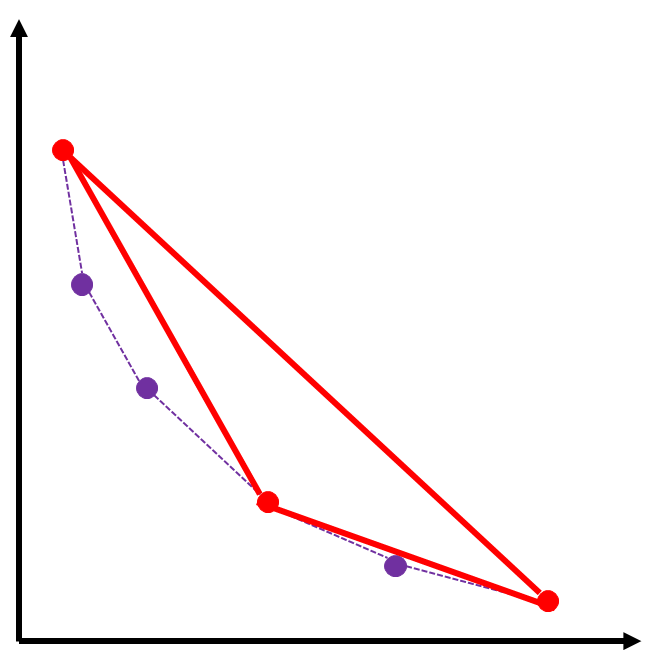
\includegraphics[width=1.0\textwidth]{figure_2D_strict.png}    
    \caption{Bounded polytope $\mathbb{P}$}
    \label{figure_illustrating_infinite_polytope_is_better_1polytope}
    \end{subfigure}
    ~
    \begin{subfigure}{0.23\textwidth}
        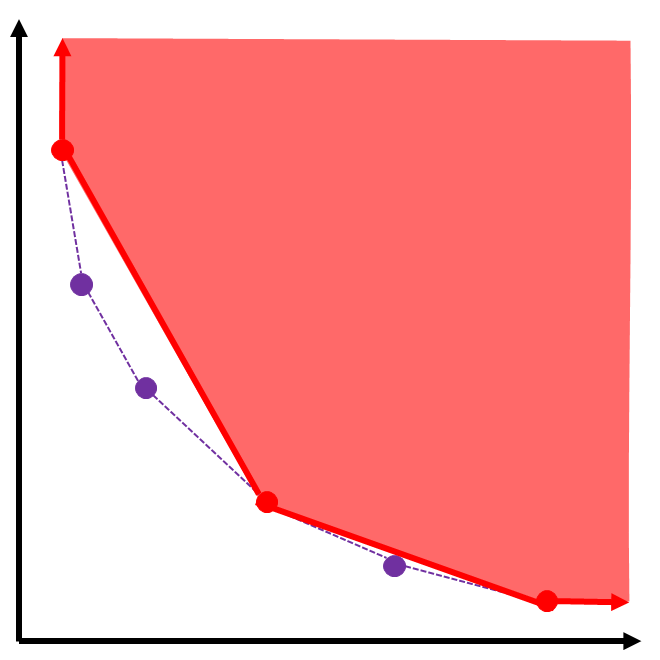
\includegraphics[width=1.0\textwidth]{figure_2D_relaxed.png}
        \caption{Infinite polytope $\mathbb{P}'$}
        \label{figure_illustrating_infinite_polytope_is_better_2envelope}
    \end{subfigure}
    ~
    \begin{subfigure}{0.23\textwidth}
        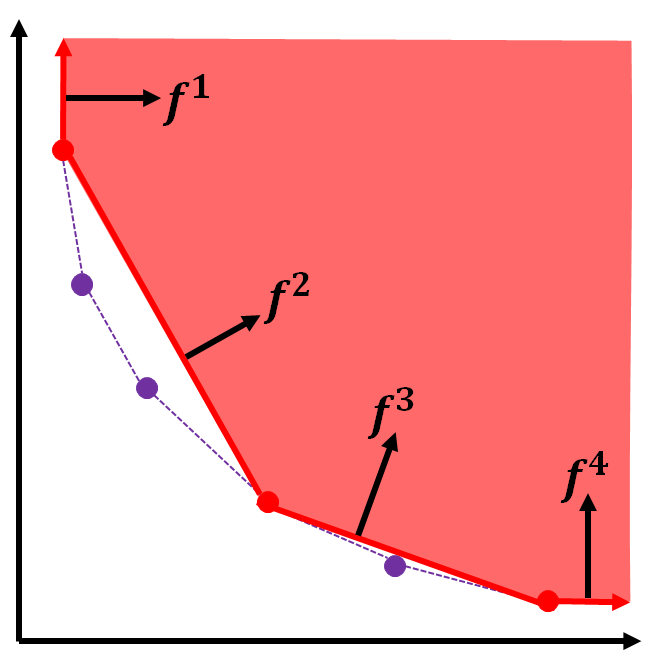
\includegraphics[width=1.0\textwidth]{figure_2D_normal.png}
        \caption{False facets}
        \label{figure_illustrating_infinite_polytope_is_better_3normal}
    \end{subfigure}
    ~
    \begin{subfigure}{0.23\textwidth}
        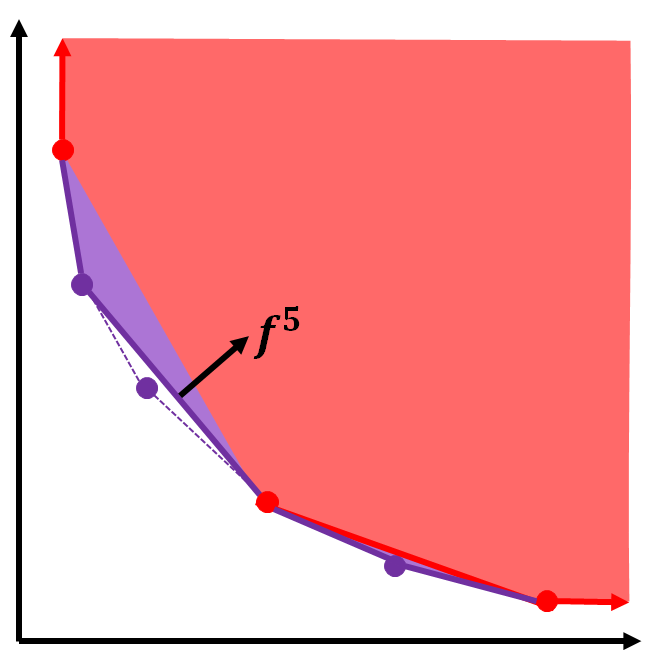
\includegraphics[width=1.0\textwidth]{figure_2D_normal_next.png}
        \caption{Iterative discovery}
        \label{figure_illustrating_infinite_polytope_is_better_4iterative}
    \end{subfigure}
\caption{\footnotesize{A 2-Dimensional illustration of the \emph{Normals Method} described in Section~\ref{subsection_general_counter_exaple}. (a) Shows 3 vertices which are (conceptually) due to STTs, that span a bounded red triangle, $\mathbb{P}$. Purple vertices denote additional (non-STT) vertices that we are unaware of, at this point. (b) shows the relaxed polytope $\mathbb{P}'$, of all points $A$ such that $\exists P \in \mathbb{P}: \forall i: P_i \le A_i$. $\mathbb{P}'$ has the same vertices as $P$, but only the facets of the lower-envelope of $\mathbb{P}$, as in this example. $\mathbb{P}'$ may gain axes-parallel facets. (c) We solve the LP in directions according to each normal vector $f^{i}$ to one of the facets of $\mathbb{P}'$. On a ``true'' facet the LP solution will not be better than expected, as for $f^{1}$ and $f^{4}$ in this illustration. However, if the facet is ``false'', the LP solution would be strictly better, revealing a new purple vertex, as for $f^{2}$ and $f^{3}$. Multiple normals may reveal the same vertex but only in $3$ dimensions and higher, see also Figure~\ref{figure_sage_3D_example}. By scanning all the facets of $\mathbb{P}'$ we determine if there are non-STT vertices, or not. (d) If we found new vertices, we can re-define the polytope and re-apply the method to search additional vertices as exemplified by the normal $f^5$.}}
\label{figure_illustrating_infinite_polytope_is_better}
\end{figure}

\begin{figure}[ht]
    \centering
    \begin{subfigure}{0.4\textwidth}
        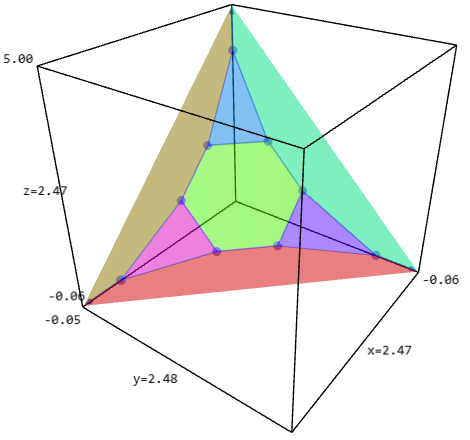
\includegraphics[width=1.0\textwidth]{figure_sage_3D_example1.png}
    \caption{Without $[0.5,0.5,0.5]$}
    \end{subfigure}
    ~
    \begin{subfigure}{0.4\textwidth}
        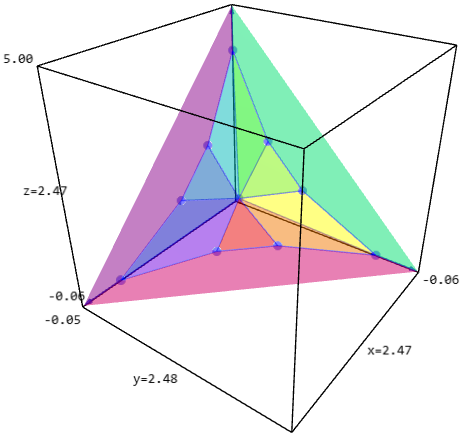
\includegraphics[width=1.0\textwidth]{figure_sage_3D_example2.png}
        \caption{With $[0.5,0.5,0.5]$}
    \end{subfigure}
\caption{\footnotesize{A 3-dimensional illustration of how the \emph{Normals Method} described in Section~\ref{subsection_general_counter_exaple} may find a single vertex for multiple false facets. The figures were produced with \emph{Sage}. 
(a) $7$ Facets of the lower envelope of the convex hull of a set of $9$ integer vertices $A = \{(4,0,0),(0,4,0),(0,0,4),(0,1,2),(0,2,1),(1,0,2),(1,2,0),(2,0,1),(2,1,0)\}$.
(b) By adding to $A$ an extra vertex $(0.5,0.5,0.5)$, $4$ of the facets turn out to be false, while every vertex remains a vertex. In both figures, each facet has its own (arbitrary) color.} The vertices in this example are not related to STTs, since the smallest ``authentic'' example is $7$-dimensional.}
\label{figure_sage_3D_example}
\end{figure}




Given the $N$ known vertices induced by STTs, we can compute the facets of $\mathbb{P}'$, and solve the LP in the direction of the normal to each facet. If the facet is ``true'', then the solution would yield an optimum whose value is equal to the value of each of the STTs that span this facet. However, if the facet is ``false'', because it ``shaves off'' vertices that we ignored, then we will find a solution that is strictly better than any of the STTs that span the false facet, whose value is strictly better than the value of each of the STTs that span this facet, and this is why we work with $\mathbb{P}'$ rather than $\mathbb{P}$.  Observe that a false facet may hide many vertices, but every normal can reveal at most one new vertex when we solve the LP in its direction.\footnote{Assuming ``general position'', that is, no set of unknown vertices spans a face that is parallel to a false facet. Otherwise, a deterministic solver will still only find one vertex, but randomization may allow finding more.} We can theoretically find all the hidden vertices by iteratively refining the search, such that whenever a new vertex is found, we compute the new facets and solve the LP in the direction of the corresponding new normal vectors. We can repeat this until all the facets are determined to be true facets. Note that in the first iteration, every facet is due to STT vertices, hence there are multiple optimal STTs for the normal of a facet (exactly those that span the facet). This explains why in Section~\ref{subsection_specific_counter_example} our analysis determines multiple optimal STTs (revisit Figure~\ref{figure_case_analysis}), and more specifically, each point in the facet satisfies the equality $D \cdot w = 30$ where $D$ is the LP depths-vector and $w = [3,2,0,2,3,3,10]$ is the normal, which tells us in advance that the optimal LP value for the points induced by STTs is $30$. Note also that for $n \ge 3$, multiple normals may result in the same new vertex, as illustrated in Figure~\ref{figure_sage_3D_example}.









\begin{definition}[Primary Directions]
\label{definition_primary_direction_terminology}
We refer to each normal to a facet of the STT induced polytope as a \emph{primary direction}.
\end{definition}

Armed with the normals method, all that remains is to enumerate all the STTs, compute their depths-vectors as our $N$ vertices, convert from vertices to facets, enumerate the facets and for each solve the LP and check if the optimum is strictly better than was expected. This is not trivial, and is computationally demanding, therefore we were only able to run it for topologies of size $n \le 8$. We exhausted all possible topologies up to this size, and detail the high-level results in the caption of Figure~\ref{figure_all_trees_up_to_n8}. See Table~\ref{table_trees_summary_analysis_vertices_etc_FEW} and Table~\ref{table_trees_summary_analysis_vertices_etc_FULL} for the detailed results. The computation was done in \emph{Sage}, and in particular
we used sage to enumerate the facets of the polytope defined as the convex hull of the STTs.
%the conversion from vertices to facets was done blackbox-wise by defining the polytope by its collection of vertices and then enumerating over its facets. 
For more on the code, see Appendix~\ref{appendix_section_code}. Due to the computational complexity of converting vertices to facets, we were unable to finish an iterative scan for all the possible vertices. To clarify, we were able to fully scan all the primary directions for each topology, and determine new non-integer vertices in seven of them. However, we did not have enough resources to compute the new facets when taking into account the newly found vertices for the topologies with $8$ nodes.
%due to inability to allocate memory. 
This failed even when only $2$ new vertices were found. We were only able to run this second phase on the topology with $7$ nodes, and for it we determined that no additional new vertices exist. (The second phase had $6385$ normals, compared to $6364$ primary directions.)

In general, many of the vertices, and the primary directions, may be symmetric. Symmetries arise due to automorphisms of the topology. If $\pi: U \to U$ is an automorphism, then we can define an automorphism on the $(X,Z,D)$-space by mapping indices according to $\pi$. For example, it maps $D_i \to D_{\pi(i)}$ and $X_{ij} \to X_{\pi(i),\pi(j)}$. Since the ``names'' of the nodes are arbitrary, it is clear why a vertex $P$ translates by $\pi$ to another vertex $P'$, and we say that $P$ and $P'$ are \emph{symmetric} to each other. Note that $P$ and $P'$ have the same coordinate values, permuted by $\pi$. There are additional cases where primary directions can look symmetric, see Remark~\ref{remark_pseudo_symmetry}.


\begin{table}[!t]%[!ht]
    \scriptsize
    \begin{center}
    \begin{tabular}{|c|c|c|c|c|c|l|l|}

    \hline
    \begin{tabular}{@{}c@{}}Topology \\ $U_{(n,i)}$ \end{tabular} &
    STTs &
    \begin{tabular}{@{}c@{}}Primary \\ Directions \end{tabular} &
    \begin{tabular}{@{}c@{}}False \\ Facets\end{tabular} &
    \begin{tabular}{@{}c@{}}Frac \\ Vs\end{tabular} &
    \begin{tabular}{@{}c@{}}Frac Vs \\ Classes\end{tabular} &
    \begin{tabular}{@{}c@{}}$D$-space \\ denom. \end{tabular} &
    \begin{tabular}{@{}c@{}}$XZD$-space \\ denom. \end{tabular} \\
    \hline
    \hline
    (3,0) & \ \ \ \ 5 & \ \ \ \ 9 & \ \ 0 & . & . &\{1\} & \{1\} {*} \\
    \hline
    (4,0) & \ \ \ 14 & \ \ \ 32 & \ \ 0 & . & . &\{1\} & \{1\} {*} \\
    \hline
    (4,1) & \ \ \ 16 & \ \ \ 32 & \ \ 0 & . & . &\{1\} & \{1\} {*} \\
    \hline
    (5,0) & \ \ \ 42 & \ \ 145 & \ \ 0 & . & . &\{1\} & \{1, 2, 3\} {*} \\
    \hline
    (5,1) & \ \ \ 51 & \ \ 152 & \ \ 0 & . & . &\{1\} & \{1\} {*} \\
    \hline
    (5,2) & \ \ \ 65 & \ \ 161 & \ \ 0 & . & . &\{1\} & \{1\} {*} \\
    \hline
    (7,3) & \ \ 662 & \ 6364 & \ 39 & 9 & 2 & \{1, 2\} & \{1, 2\} \\
    \hline
    (8,4) & \ 2416 & 48291 & 362 & 65 & 38 & \{1, 2\} & \{1, 2, 3\} \\
    \hline
    (8,5) & \ 2952 & 56376 & 120 & 2 & 1 & \{1, 2\} & \{1, 2, 3\} \\
    \hline
    (8,6) & \ 2802 & 56724 & \ 10 & 2 & 1 & \{1, 2\} & \{1, 2, 3, 4\} \\
    \hline
    (8,11) & \ 3988 & 54201 & \ 78 & 18 & 4 & \{1, 2\} & \{1, 2\} \\
    \hline
    (8,12) & \ 3332 & 56404 & 528 & 60 & 24 & \{1, 2\} & \{1, 2, 3\} \\
    \hline
    (8,13) & \ 4076 & 65733 & 946 & 28 & 4 & \{1, 2\} & \{1, 2\} \\
    \hline
    \end{tabular}
    \end{center}
    \caption{
    \footnotesize{\largeTablecaption{Summary of all tree topologies up to $n \le 5$ nodes and those with non-STT $D$-space vertices up to $n \le 8$ (for more topologies, see Table~\ref{table_trees_summary_analysis_vertices_etc_FULL}).}}}
    \label{table_trees_summary_analysis_vertices_etc_FEW}
\end{table}




\begin{figure}
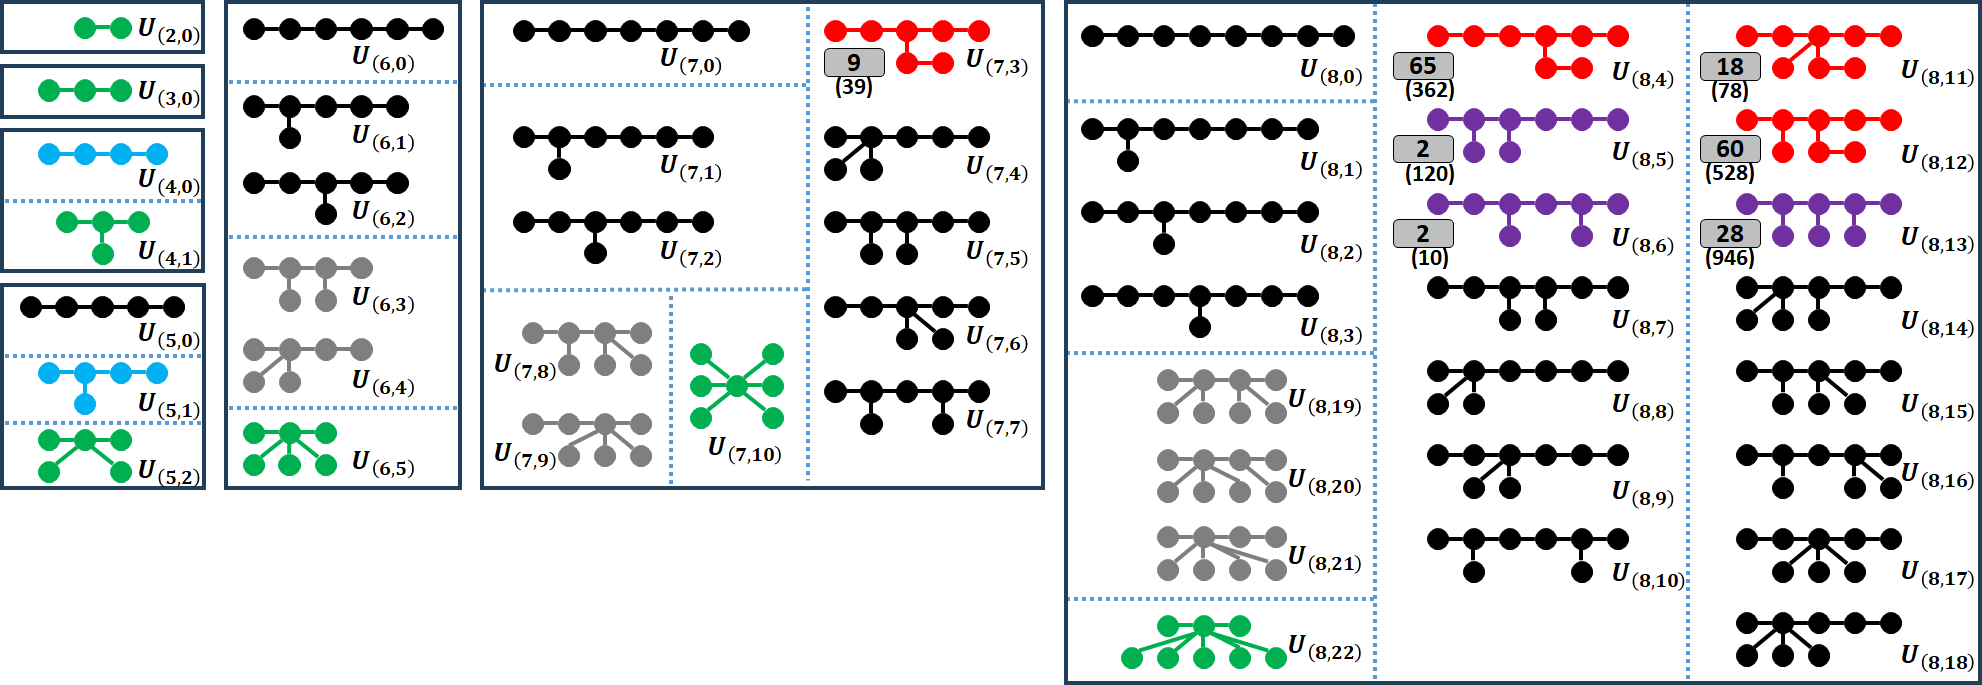
\includegraphics[width=1.0\textwidth]{figure_all_trees_up_to_n8.png}
\caption{\footnotesize{All tree topologies with $2 \le n \le 8$ nodes, 47 in total. Each tree is named $U_{(n,i)}$ where $n$ is its number of nodes and $i$ is a running index, over non-increasing diameter. For example, $U_{(n,0)}$ is always the path over $n$ nodes and the last among $U_{(n,i)}$ is the star with $n$ nodes. The number of trees for each $n$ is also known as OEIS sequence A000055 (see: https://oeis.org/A000055). Rectangles group by size $n$, and dashed lines divide by diameter within each group. Color scheme: Green trees are stars, analytically proven to have only integer vertices in $(X,Z,D)$-space. 
Blue trees were also verified to have only integer vertices in $(X,Z,D)$-space, with computer assistance. Black trees only have integer vertices in $D$-space, but have non-integer vertices in $(X,Z,D)$-space, this is further discussed in Section~\ref{subsection_with_and_without_z_fourier_motzkin}.
Gray trees may be either blue or black, it was infeasible to verify. Red and purple mark trees with non-integer vertices in $D$-space, i.e., counter-example vertices. The red trees are the unique such tree for $n=7$ and its extensions to $n=8$ (Definition~\ref{definition_extended_graph}), while purple trees are additional topologies that cannot be extended from the red tree with $7$ nodes. The number of non-integer vertices is written in a gray box near each tree, and in parenthesis is the number of false facets (or, primary directions) by which we found these vertices.}}
\label{figure_all_trees_up_to_n8}
\end{figure}

We follow with some additional information on the topology $U_{(7,3)}$ used in the proof of Theorem~\ref{theorem_non_integer_optimum_long_star}. Its LP has a total of $39$ false facets which correspond to $9$ non-integer vertices. By the automorphism symmetry of the topology it is natural that these numbers are divisible by $3$. There are $7$ normals, such that one of them has 3 symmetric copies and each of the other six has 6 copies. These normals are (the first was used in Theorem~\ref{theorem_non_integer_optimum_long_star}): $w = (3, 2, 0, 2, 3, 3, 10)$, $(14, 6, 0, 10, 32, 5, 7)$, $(16, 6, 0, 11, 34, 4, 8)$, $(39, 11, 0, 6, 21, 4, 8)$, $(18, 6, 0, 10, 36, 5, 7)$, $(18, 5, 0, 3, 6, 4, 5)$, $(9, 4, 0, 7, 22, 4, 5)$. Information about other trees is summarized in Table~\ref{table_trees_summary_analysis_vertices_etc_FEW}.

We conclude our findings with an interesting remark.

\begin{definition}[Partially Integer Vertex]
\label{definition_partially_integer_vertex}
We say that an $(X,Z,D)$-vertex is \emph{partially integer} if its $D$ coordinates are all integer, but at least one $X$ coordinate is non-integer.
\end{definition}


\begin{remark}[New vertices are half-integer]
\label{remark_new_vertices_are_non_integer_half_integer_only}
Partially integer vertices exists, an example is given in Figure~\ref{figure_Example_partially_interger_vertex}. Therefore, the normals method may technically find partially integer vertices which do not correspond to STTs. Indeed, while Property~\ref{property_integer_domination} says that STT-vertices dominate other integer points, it is with respect to fully integral points in $(X,Z,D)$-space.

However, interestingly every new $D$-space vertex that we were able to find has non-integer depths. Partially integer vertices that we found are always projected to non-vertices in $D$-space. Moreover, all depths are half-integer, that is, have coordinates that are $0$ or $\frac{1}{2}$, modulo $1$ (some coordinates may be integer, but not all of them). Is all of this an artifact of small sizes ($n \le 8$), like the fact that all the polytopes are integer for $n \le 4$, or is it an inherent property?
\end{remark}


\begin{example}
\label{figure_Example_partially_interger_vertex}
The smallest example for a partially integer vertex (Definition~\ref{definition_partially_integer_vertex}) is for $n=6$, see $P_1$ in Equation~(\ref{equation_partially_integer_vertex}). We find $P_1$ when solving the LP for the path topology, in some general $(X,Z,D)$-direction.\footnote{
The order of LP variables is defined in the code, in the function named ``\_construct\_dictionaries\_PRIMAL'' of the \emph{SearchTreeUtilities} class. The direction according to their order is [0, 5, 5, 1, 2, 3, 1, 4, 1, 1, 3, 3, 1, 4, 2, 2, 3, 5, 3, 1, 1, 3, 5, 4, 2, 2, 6, 0, 2, 1, 5, 3, 3, 1, 5, 4, 4, 5, 3, 2, 1, 6, 3, 5, 2, 3, 4, 5, 3, 2, 2, 1, 0, 3, 5, 2].} The depths-vector of $P_1$ is dominated by the STT (BST) $[2,1,2,0,1,2]$. In other cases (not shown) the depths are dominated by a convex combinations of more than one STT. For $n \le 5$, only the path topology has non-integer vertices, and each has a non-integer $D$ coordinate (and is projected to a non-vertex in $D$-space).

{\scriptsize
\begin{equation}
\label{equation_partially_integer_vertex}
P_1 = \frac{1}{2} \cdot 
\begin{bmatrix}
. & 2 & 0 & 0 & 0 & 0 \\
0 & . & 1 & 0 & 0 & 2 \\
2 & 1 & . & 1 & 1 & 0 \\
1 & 1 & 1 & . & 1 & 2 \\
1 & 0 & 0 & 1 & . & 2 \\
0 & 0 & 2 & 0 & 0 & . \\
\hline
4 & 4 & 4 & 2 & 2 & 6 \\
\end{bmatrix}
% %% Another example, in the larger topology $U_{8,6}$ that extends PATH(6), and also has non-integer vertices. No need to show it, saving some space and cluttering.
% ~
% Q_2 = \frac{1}{2} \cdot 
% \begin{bmatrix}
%  . & 1 & 0 & 0 & 0 & 1 & 1 & 2 \\
% 1 & . & 1 & 1 & 1 & 0 & 1 & 0 \\
% 1 & 1 & . & 1 & 1 & 1 & 1 & 1 \\
% 0 & 1 & 1 & . & 1 & 1 & 1 & 1 \\
% 0 & 0 & 0 & 1 & . & 1 & 0 & 1 \\
% 0 & 0 & 0 & 0 & 1 & . & 0 & 0 \\
% 0 & 1 & 0 & 0 & 0 & 0 & . & 1 \\
% 0 & 0 & 0 & 1 & 0 & 0 & 0 & . \\
% \hline
% 2 & 4 & 2 & 4 & 4 & 4 & 4 & 6 \\
% \end{bmatrix}    
\end{equation}
}
\end{example}


\subsection{Integrality Gap - Lower Bounds}
\label{subsection_integrality_gap}
A lower bound of $\frac{60}{59}$ on the integrality gap of the LP follows from Theorem~\ref{theorem_non_integer_optimum_long_star}. For a tighter lower bound on the integrality gap, we can study all the non-integer vertices in all seven small topologies that have such vertices.

\begin{lemma}
\label{lemma_additive_gap}
Given a fixed topology $U$, let $\mathbb{D} = \{ D^1,\ldots,D^N \} $ be all the $D$-space vertices induced by STTs, and let $\mathbb{S} = \{S^1,\ldots,S^M \}$ be additional vertices of the $D$-space projection of the LP polytope, where each $S^i$ is found by solving the LP in the primary directions $h^{i,1},\ldots,h^{i,{k_i}}$ for some $k_i \ge 1$. Denote $\Delta \equiv \max \{ \min_{A \in conv^+(\mathbb{D})}(A \cdot f) - \min_{B \in conv^+(\mathbb{D} \cup \mathbb{S})} (B \cdot f) \mid \forall i: f_i \ge 0 \wedge \sum_{i=1}^{n}{f_i} = 1 \}$ (the largest additive gap), where $conv^+$ is a convex combination over a set of points, and positive rays.
Then if $\Delta > 0$, it is achieved for some $i,j,k$ such that $B=S^i$, $f = \hat{h}^{i,j}$ and $A = D^k$, where hat represents normalization to a sum of one, and $D^k$ is on the false facet of $conv^+(\mathbb{D})$ whose normal is $h^{i,j}$. (Recall Section~\ref{subsection_general_counter_exaple}.)
\end{lemma}
\begin{proof}
Let $f$ be a direction (vector) that maximizes $\Delta$. The scalar product with $f$ projects the polytope $conv^+(\mathbb{D})$ to one dimension, therefore the minimum has a pre-image that is a vertex, this is $A = D^k$. Similarly, by arguing for $conv^+(\mathbb{D} \cup \mathbb{S})$ we get that $B$ can be chosen as either some $D^i$ or $S^i$. However, $D^k \cdot f \le D^i \cdot f$ for every $1 \le i \le N$, so it must be that $B = S^i$ (or else $\Delta = 0$).

Now fix $A$ and $B$, denote $C = A-B$, and let us show that we can replace $f$ by some $\hat{h}^{i,j}$, without decreasing $\Delta$ which will conclude the proof. Since $f$ is a (normal to a) separating plane that intersects $A$, in a problem of covering form,\footnote{An LP problem of the form minimize $c \cdot x$ where $Ax \ge b$, $x \ge 0$, $c \ge 0$ for vectors $x,b,c$ and matrix $A$.} by strong-duality we get that $f = \sum_{j}{\alpha_j \cdot \hat{h}^j}$ for non-negative coefficients $\alpha_j$, where $h^j$ are all the normals to facets of $conv^+(\mathbb{D})$ that contain $A$. Moreover, $\sum_j {\alpha_j} = 1$ because all of $f$ and $\hat{h}^j$ have coordinate sum of $1$. We get that:
$C \cdot f = \sum_{j}{\alpha_j \cdot (C \cdot \hat{h}^j)} \le C \cdot \hat{h}^{j^*}$ by choosing $j^*$ that maximizes the scalar product. However, since $f$ is a maximizer, we get equality, and conclude that $\hat{h}^{j^*}$ is a primary direction that maximizes $\Delta$. Finally, it must be that $\hat{h}^{j^*}$ is a normal to a false facet that contains $A$. Otherwise, it does not imply a separating plane, and therefore $A \cdot \hat{h}^{j^*} - B \cdot \hat{h}^{j^*} \le 0$, which is a contradiction.
\end{proof}

By Lemma~\ref{lemma_additive_gap} it suffices to consider only vertices and primary directions to maximize the additive gap, and in particular only check for gaps of the form: $(D^k - S^i) \cdot h^{i,j}$. By choosing for each topology the vertices $S^i$ and $D^k$, and the primary direction $h^{i,j}$ that maximize $\Delta$, we get Table~\ref{table_integrality_gaps}. Anecdotally, the largest gap for $U_{(7,3)}$ is due to the primary direction which we studied in Theorem~\ref{theorem_non_integer_optimum_long_star}. Based on the small topologies we studied, the integrality gap is at least $\frac{95}{93} \approx 1.0215$, which is much closer to $1$ (almost optimal) than to the proven upper bound of $2$. Note that maximizing the difference does not necessarily maximize the integrality gap (ratio).
% So there is room for improving the lower-bound, even on the small topologies with $n \le 8$.

%%% The following is an LP to optimize the difference, but indeed, the optima are always primary directions.
% \begin{definition}[LP for Gap Optimization]
% \label{definition_LP_for_integrality_gap}
% We assume knowledge of all the STT depths-vectors, denotes $D^1,\ldots,D^N$, and another (non-STT) vertex $P$. We determine a frequencies vector $f$ that maximizes the difference: $\min_{i}\{D^i \cdot f\} - P \cdot f$.
% \begin{enumerate}
%     \item Variables: $x$ (scalar) and $f$ (vector).
%     \item Constraints: (a) $\forall 1 \le i \le n: f_i \ge 0$; (b)  $\sum_{i=1}^{n}{f_i} = 1$; (c) $\forall 1 \le i \le N: x \le D^i \cdot f$.
%     \item Objective: maximize $x - P \cdot f$.
% \end{enumerate}
% \end{definition}

Another interesting note is that the topology $U_{(8,11)}$ extends $U_{(7,3)}$ (Definition~\ref{definition_extended_graph}), and it happens to be that the direction that maximizes the difference for $U_{(8,11)}$ is an extension of the direction that maximizes the difference for $U_{(7,3)}$.


\begin{table}[!ht]%[!ht]
    \scriptsize
    \begin{center}
    \begin{tabular}{|c|c|c|c|r|}

    \hline
    Topology $U_{(n,i)}$ & Direction & LP Value & STT Best Value & Integrality Gap \\
    \hline
    (7,3) & (3,2,0,2,3,3,10) & \ 29.5 & \ 30 & $60/59 \approx 1.0169$ \\
    \hline
    (8,4) & (9,5,0,6,11,17,5,9) & \ 93 \ \ & \ 95 & $\mathbf{95/93 \approx 1.0215}$ \\
    \hline
    (8,5) & (16,2,3,6,7,13,34,5) & 121 \ \ & 122 & $122/121 \approx 1.0083$ \\
    \hline
    (8,6) & (55,1,3,4,14,29,34,8) & 200.5 & 201 & $402/401 \approx 1.0025$ \\
    \hline
    (8,11) & (3,2,0,2,3,0,3,10) & \ 29.5 & \ 30 & $60/59 \approx 1.0169$ \\
    \hline
    (8,12) & (11,1,0,1,2,6,1,2) & \ 28.5 & \ 29 & $58/57 \approx 1.0175$ \\
    \hline
    (8,13) & (7,1,1,1,7,7,2,7) & \ 49.5 & \ 50 & $100/99 \approx 1.0101$ \\
    \hline
    \end{tabular}
    \end{center}
    
    \caption{\footnotesize{For each topology with non-STT vertices, we show a primary direction (Definition~\ref{definition_primary_direction_terminology}) that maximizes the integrality gap among all primary directions. The largest gap overall is marked in bold.}}
    \label{table_integrality_gaps}
\end{table}


\subsection{Approximation Ratio of the Root Rounding - Lower Bounds}
\label{subsection_approximation_ratio}

So far we just disproved the first (and stronger) conjecture, and studied the integrality gap of the LP. In this section we return to the original problem of STTs, and consider the rounding in Definition~\ref{definition_rounding_scheme}. We disprove Conjecture~\ref{conjecture_LP_rounding_finds_opt_STT} that claims it rounds to an optimal STT. The rounding scheme may have degrees of freedom, and we study it both when assuming the worst-case scenario (pick a worst choice) and in the best-case scenario (pick a best choice).

Interestingly, for all the seven small topologies ($n \le 8$) for which non-STT vertices were found, when solving the LP in a primary direction, there is a rounding that yields an optimal STT. At a first glance this suggests that there is hope to refine the rounding scheme to remove misleading degrees of freedom (of choosing which node to root at each iteration). However we show later in this section that  in non-primary directions we are no longer guaranteed an optimal rounding. This ``strongly'' disproves Conjecture~\ref{conjecture_LP_rounding_finds_opt_STT} by showing that the rounding scheme could be suboptimal regardless of the degrees of freedom in the rounding procedure.

Table~\ref{table_approximation_ratios} summarizes our findings for the seven topologies with non-STT vertices. We show that every topology has directions for which even the best-case rounding is sub-optimal. We also show directions with large worst-case ratios, the largest that we found, though not by an exhaustive search or analysis, is $\frac{263}{190} \approx 1.384$. This is a lower-bound on the approximation ratio of the root rounding approach.

\begin{table}[!ht]%[!ht]
    \scriptsize
    \begin{center}
    \begin{tabular}{|c|c|c|c|c|c|c|c|c|c|}

    \hline
    Topology $U_{(n,i)}$ &  \multicolumn{2} {|c|} {Direction} & OPT STT & BC STT & WC STT & BC Ratio & WC Ratio \\
    \hline
    (7, 3) & (11, 7, 0, 10, 34, 7, 11) & {*} & 184/80 & 186/80 & 220/80 & 1.0109 & 1.1957 \\
    \hline
    (8, 4) & (17, 9, 0, 10, 19, 29, 9, 17) & {*} &  277/110 & 281/110 & 339/110 & \textbf{1.0144} & 1.2238 \\
    \hline
    (8, 5) & (13, 1, 2, 4, 5, 10, 25, 4) & {*} &  154/64 & 155/64 & 178/64 & 1.0065 & 1.1558 \\
    \hline
    (8, 6) & (86, 1, 5, 6, 22, 46, 55, 13) & {*} &  552/234 & 553/234 & 658/234 & 1.0018 & 1.192 \\
    \hline
    (8, 11) & (11, 7, 0, 7, 11, 0, 10, 34) & {*} &  184/80 & 186/80 & 220/80 & 1.0109 & 1.1957 \\
    \hline
    (8, 12) & (32, 2, 0, 3, 7, 18, 3, 7) & {*} &  160/72 & 162/72 & 188/72 & 1.0125 & 1.175 \\
    \hline
    (8, 13) & 
    \begin{tabular}{@{}l@{}}(48, 6, 5, 6, 48, 48, 15, 48) \\ $+\epsilon \cdot (-1,1,1,1,-1,-1,-1,-1) $ \end{tabular}
    & {**} &  $\frac{558-\epsilon}{224 - 2\epsilon}$ & $\frac{563-6\epsilon}{224 - 2\epsilon}$ & $\frac{647-7\epsilon}{224 - 2\epsilon}$ & 1.0090 & 1.1595 \\
    \hline
    (8, 4) & (6, 3, 0, 5, 0, 18, 4, 5) & ${p}$ &  94/41 & 94/41 & 129/41 & 1 & 1.3723 \\
    \hline
    (8, 4) & (6.5, 3, 0, 5, 0, 18, 4, 5) & ${p'}$ &  190/83 & 191/83 & 263/83 & 1.0053 & \textbf{1.3842} \\
    \hline
    (8, 13) & (10, 2, 1, 2, 35, 35, 2, 10) & ${p}$  & 216/97 & 216/97 & 283/97 & 1 & 1.3102 \\
    \hline
    \hline
    \end{tabular}
    \end{center}
    \caption{\footnotesize{For each topology whose LP finds non-STT vertices, we show directions and approximation ratios of the best-case (BC) and worst-case (WC) root rounding. The first $7$ rows give one entry per topology with a direction in which even the best-case is sub-optimal. The next rows show additional directions for which the worst-case is among the largest that we found. Directions marked ${*}$/${**}$ were found by the LP in Definition~\ref{definition_LP_for_approximation_gap}, ${p}$ marks primary directions that give large ratios, and ${p'}$ marks a small variation to increase the largest gap we found among primary directions. Remark~\ref{remark_int_gap_zero_must_perturb} explain why in the case of ${**}$ we perturb the nice integer direction by $\epsilon$.}}
    \label{table_approximation_ratios}
\end{table}




In the remainder of this section we detail the following: Theorem~\ref{theorem_rounding_the_vertex} demonstrates an explicit worst-case rounding of the optimum shown in Figure~\ref{figure_explicit_counter_example} (for Theorem~\ref{theorem_non_integer_optimum_long_star}), that gives an approximation ratio of $\frac{62}{53} \approx 1.170$. Then we explain how to find directions in which the root rounding is sub-optimal and where the directions in Table~\ref{table_approximation_ratios} come from.


\begin{theorem}
\label{theorem_rounding_the_vertex}
The approximation ratio of root rounding (Definition~\ref{definition_rounding_scheme}) is at least $\frac{62}{53}$.\\ (As shown in Table~\ref{table_approximation_ratios}, other (numerical) examples show that it is can be even worse.)
\end{theorem}

\begin{proof}
Consider the case of Theorem~\ref{theorem_non_integer_optimum_long_star}, of weights $w = (3,2,0,2,3,3,10)$ and the non-integer solution described in Figure~\ref{figure_explicit_counter_example}. We show a set of choices that round this solution to an STT with depths-vector $D = (4, 3, 2, 3, 4, 1, 0)$. Then its LP value is $w \cdot D = 12+6+0+6+12+3 = 39$, compared to the best STT whose value is $30$. By Remark~\ref{remark_depth_off_by_one}, the approximation ratio is $\frac{39 + \sum{w_i}}{30 + \sum{w_i}} = \frac{62}{53} \approx 1.170$.

We now round step by step, for each connected component $C$ throughout the process.
\begin{enumerate}
    \item Initially, $C = \{1,\ldots,7\}$ (whole tree): since $X_{7i} = \frac{1}{2}$ for each $i=1,\ldots,6$, we can choose the root $r=7$. $C \setminus \{r\}$ remains a single connected component.

    \item $C = \{1,\ldots,6\}$: since $X_{6i} \ge \frac{1}{2}$ for each $i=1,\ldots,5$, we can choose the root $r=6$. $C \setminus \{r\}$ remains a single connected component, now it is a path.

    \item $C = \{1,\ldots,5\}$: while $X_{3i} = 0$ for $i=1,2,4,5$, choosing $r=3$ as the root satisfies the condition because $X_{24}=X_{25}=X_{41}=X_{42}=\frac{1}{2}$. $C \setminus \{r\}$ now has two connected components.

    \item $C = \{1,2\}$: since $X_{21} = \frac{1}{2}$ we can root at $2$. This leaves a singleton subtree $C \setminus \{2\} = \{ 1 \}$.

    \item $C = \{4,5\}$: since $X_{45} = \frac{1}{2}$ we can root at $4$. This leaves a singleton subtree $C \setminus \{4\} = \{ 5 \}$.
\end{enumerate}
Combining all of the above yields an STT whose  depths-vector $(4, 3, 2, 3, 4, 1, 0)$.
\end{proof}

We could refine root rounding by solving the LP recursively for each connected component after picking the root, instead of rounding always based on the same one-time solution. In the example of Theorem~\ref{theorem_rounding_the_vertex} it does help, because $7$ is a root of some optimal STT with respect to $w$, and we know that when the topology has size $n \le 6$ the LP approach is optimal. However, this refined rounding does not generally circumvent the problem, since we show next that we might pick the root sub-optimally. When this happens, the resulting STT is suboptimal even if we can improve our choices and the overall approximation ratio by constructing the subtrees better.

\medskip

In the remainder of this section, we discuss how to find directions 
for which root rounding has a
relatively large approximation ratio. First let us discuss the best-case rounding. As noted, to ensure a gap, even under the refined (iterated) root rounding, it is sufficient to ensure an empty intersection between the set of candidate roots, which we denote by $R$, and the set of roots of optimal STTs, which we denote by $O$.\footnote{Note that if we could guarantee a rounding that shares a root with an optimal solution, the refined (iterated) root rounding would give an optimal STT.} It  requires  to solve an LP $O(n)$ times instead of once, but the running time will remain polynomial.

As a first step, we can look for a primary direction for which $O \setminus R \ne \emptyset$. Then we can variate slightly the primary direction to ensure that all the optimal STTs have a root from $O \setminus R$. This naive approach does not always work, and by checking the sets $O$ and $R$ for each primary direction, we find multiple such directions only for the topologies $U_{(8,4)}$ and $U_{(8,13)}$.
%[extra details, omitted for brevity] Interestingly, in the case of $U_{(8,4)}$ whenever $O$ and $R$ differ we have that $O = \{3,4,6\}$, $R = \{4,5,6\}$. This is just a coincidence, for $U_{(8,13)}$ there are multiple different cases of partial intersections.
Moreover, primary directions are only special because they let us find a non-STT vertex, but they do not necessarily maximize the approximation ratio. To be more comprehensive, we can define an LP to find the unknown direction $f$ that maximize the distance between a non-STT vertex $P$ and all the STTs that root rounding can reach from it. Formally:

\begin{definition}[LP for Best-Case Approximation Ratio]
\label{definition_LP_for_approximation_gap}
Assume knowledge of all the depths-vectors of STTs, denoted by $D^1,\ldots,D^N$, and another (non-STT) vertex $P$. Also, let $S^1,\ldots,S^M$ be the set of all STTs we can get by root roundings of $P$. Ideally we aim to determine a frequencies vector $f$ that maximizes the separation: $\min_{i}\{S^i \cdot f\} - \min_{i}\{D^i \cdot f\}$, subject to $\min_{i}\{D^i \cdot f\} \ge P \cdot f$. For reason we explain later, we guess and fix the minimizer for $\min_{i}\{D^i \cdot f\}$, denoted by $D'$.

The LP: Maximize $x - D' \cdot f$, for the variables $x$ (scalar) and $f$ (vector), subject to:
\begin{enumerate}
    \item Frequencies: (i) $\forall 1 \le i \le n: f_i \ge 0$;\ \ \ \ (ii)  $\sum_{i=1}^{n}{f_i} = 1$.
    \item Hierarchy: (iii) $P \cdot f \le D' \cdot f$;\ \ \ \ (iv) $\forall 1 \le i \le N: D' \cdot f \le D^i \cdot f$.
    \item Technical helper variable: (v) $\forall 1 \le i \le M: x \le S^i \cdot f$.
\end{enumerate}
\end{definition}

Ideally we would define two helper variables $x$ and $y$ such that the constraints give us $x = \min_{i}\{S^i \cdot f\}$ and $y = \min_{i}\{D^i \cdot f\}$, and then maximize $x-y$. We defined $x$, but cannot do it for $y$. Since we maximize $x-y$ attempting to do it by requiring $\forall 1 \le i \le N: y \le D^i \cdot f$ will simply lead to an unbounded small value for $y$ (or the minimum possible if we artificially bound it from below, say with $y \ge 0$). For this reason, we compromised and solved for each option of $D' \in \{D^1,\ldots,D^N\}$. The LP has no solution for some wrong guesses of $D'$, but this does not affect us. However, solving this large number of instances is highly inefficient, and is feasible only for small topologies. We obtained from this LP the directions marked by ${*}/{**}$ in Table~\ref{table_approximation_ratios}. Note that just like with the integrality gap, we optimized the direction $f$ to maximize a difference rather than the actual approximation ratio, so the actual lower bound may be larger.

\begin{remark}
\label{remark_int_gap_zero_must_perturb}
Definition~\ref{definition_LP_for_approximation_gap} technically allows for $P \cdot f = D' \cdot f$. Then there is no integrality gap, and when we solve the original LP (Definition~\ref{definition_LP_program}) we may find an STT induced vertex, so that we do not even need to approximate, in contrast to what we aim to find. This, in fact, happens when we run the solver on the topology $U_{(8,13)}$, see the direction marked in ${**}$ in Table~\ref{table_approximation_ratios}. To overcome this issue, we replace constraint (iii) by the constraint $P \cdot f + \epsilon \le D' \cdot f$ for a small $\epsilon > 0$, say $0.001$, to truly guarantee an approximation ratio that is larger than $1$.
\end{remark}

Moving on to maximizing the worst-case approximation ratio, we can try a similar LP as in Definition~\ref{definition_LP_for_approximation_gap}. In this case, using the same notations, we would like to maximize $\max_{i}\{S^i \cdot f\} - \min_{i}\{D^i \cdot f\}$. The problem here is that we cannot define the helper-variable $x$ such that modifying its constraints gives $x = \max_{i}\{S^i \cdot f\}$ while simultaneously maximizing $x - D' \cdot f$. Instead, we can guess an $S' \in \{ S^1,\ldots,S^M\}$ that maximizes the expression, similar to our guess of $D'$. The problem is that we get an additional slowdown factor of $M$, since we now solve $M \cdot N$ instances (one per guess of $D'$ and $S'$). For the small topologies we already have $M \approx 30$, depending on the vertex that we round.

At this point, it does not seem too important to pin-point the exact approximation ratios for only a few specific small topologies. So, as a crude replacement, we may check each primary direction for its worst-case rounding. This is feasible, and we find some larger ratios compared to the best-case roundings, as should be expected. The primary directions for topologies $U_{(8,4)}$ and $U_{(8,13)}$ break the $1.3$ barrier, 
they appear in Table~\ref{table_approximation_ratios} marked with ${p}$. To emphasize that these primary directions do not maximize the approximation ratio, we also show a deviation from one of the directions, marked with ${p'}$ in the table. It is possible to deviate from a primary direction by not too much while maintaining the same vertex solution of the LP. Thus, by considering some random deviations we were able to find an improved direction. We emphasize that this is likely not the direction that maximizes the approximation ratio as our search was not exhaustive.